\section{Benchmark 3: Integrated Circulation, Energy, and Helicity}

To further validate the physical consistency of the vortex ring as a photon analog in VAM, we compute three global quantities:

\begin{itemize}
    \item \textbf{Circulation} $\Gamma$
    \item \textbf{Vorticity energy} $U_{\text{vortex}}$
    \item \textbf{Helicity} $H = \int \vec{v} \cdot \vec{\omega} \, d^3x$
\end{itemize}

These quantities relate directly to the observable properties of electromagnetic and gravitational fields in the model.

\subsection{Circulation}

Circulation around a closed loop $\mathcal{C}$ enclosing the vortex ring is defined as:

\begin{equation}
\Gamma = \oint_{\mathcal{C}} \vec{v} \cdot d\vec{\ell}
\end{equation}

For an ideal thin-core vortex ring, $\Gamma$ is a topologically quantized constant. In the VAM interpretation, circulation defines the discrete quantum of swirl that corresponds to elementary excitation modes — such as photons or charged particles.

\subsection{Swirl Energy}

The total kinetic energy stored in the vortex ring is computed via:

\begin{equation}
U_{\text{vortex}} = \frac{1}{2} \rho_{\text{\ae}} \int |\vec{v}(\vec{x})|^2 \, d^3x
\end{equation}

This quantity determines the inertial response of the structure and, in the case of fermionic knots, contributes to the gravitational mass through time dilation:

\begin{equation}
dt = dt_{\infty} \sqrt{1 - \frac{U_{\text{vortex}}}{U_{\text{max}}}}
\end{equation}

\subsection{Helicity}

The helicity of the vortex ring is defined as:

\begin{equation}
H = \int \vec{v} \cdot \vec{\omega} \, d^3x
\end{equation}

This is a topological invariant under ideal flow conditions. Nonzero helicity indicates a knotted or linked structure — essential for representing electric charge in VAM. In the case of a chiral toroidal vortex, $H \neq 0$ and its sign determines polarization:

\begin{itemize}
    \item $H > 0$ \quad $\Rightarrow$ Right-circularly polarized photon
    \item $H < 0$ \quad $\Rightarrow$ Left-circularly polarized photon
\end{itemize}

\begin{figure}[H]
    \centering
    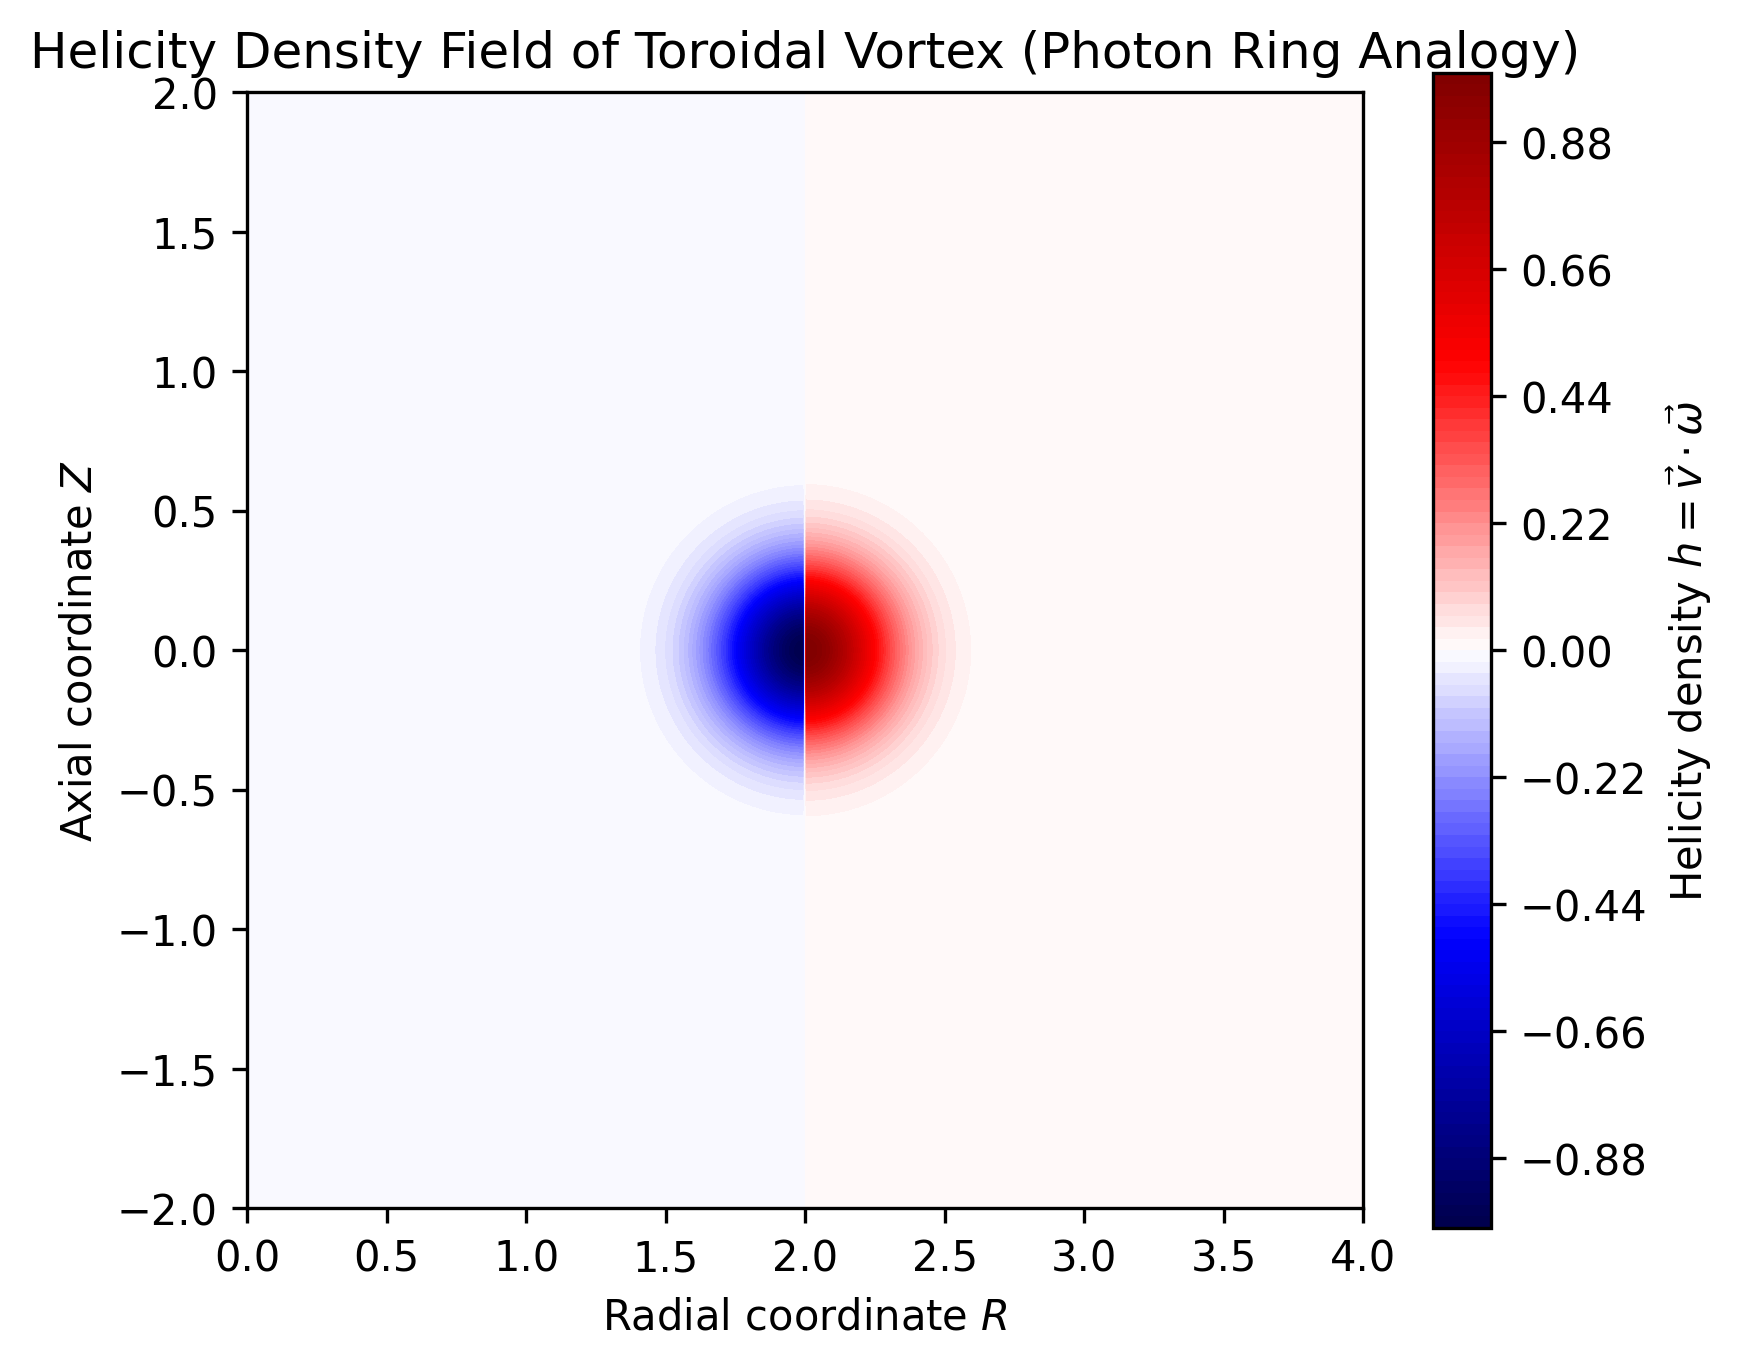
\includegraphics[width=0.6\textwidth]{helicity_ring_integration.png}
    \caption{Integrated helicity $H$ for a vortex ring configuration. This scalar value distinguishes topologically active (charged or polarized) vortex states from null configurations like neutrinos or vacuum modes.}
\end{figure}

\subsection{Physical Interpretation}

In the VAM framework:

\begin{align*}
q &\propto H \quad \text{(electric charge)} \\
m &\propto U_{\text{vortex}} \quad \text{(gravitational mass)} \\
S &\propto \Gamma \quad \text{(spin quantum number)}
\end{align*}

This completes the identification of vortex-derived quantities with fundamental properties in the Standard Model. The vortex ring thus satisfies the field, geometric, and dynamical benchmarks required to model elementary bosons.

